Overwhelmed with genomic data, biologists are facing a wealth of easily accessible sequence data but there is little use in this data without verified experimental annotation. Especially interesting, but also difficult to obtain and consequently sparse is the functional annotation of proteins, which helps to understand life at the molecular level and is e.g.~important in understanding and curing diseases. Homology-based function prediction fills the gap by transferring verified annotations to related proteins of unknown function under the reasonable assumption that function is at least partly conserved between homologs -- homologs to a kinase will likely still function as kinases but  with different substrates. A generic procedure is shown in figure \ref{fig:function_transfer}. We implemented such a homology-based approach with HypfuNN, our Homology-based protein function predictor utilizing neural networks. This working paper first describes details of the implementation, then presents the results of a 10 times 10-fold crossvalidation on a dataset of 2,815 protein sequences annotated with the HPO ontology of human phenotypes~\citep{Koehler2014} collected from public databases.

\begin{figure}[!hb]
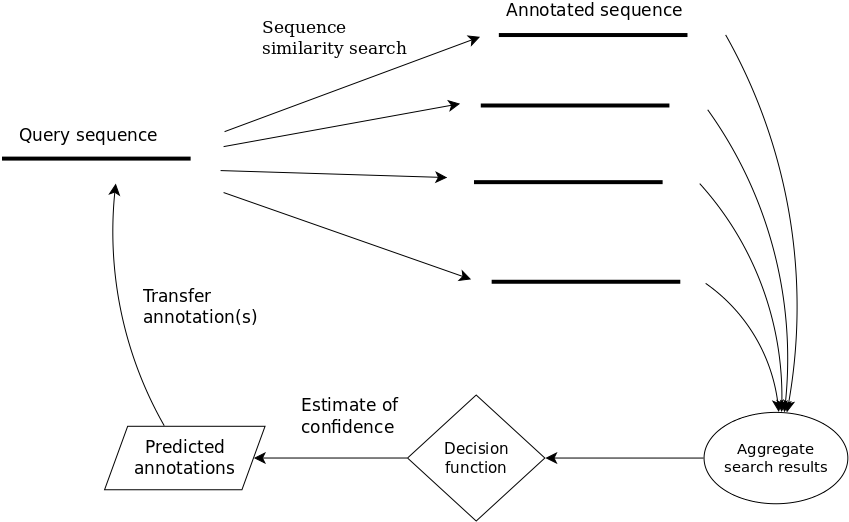
\includegraphics[width = 0.4\textwidth]{figures/function_transfer.png}
\caption{Homologs to a query sequence can be detected via similarity search, e.g.~blast, and annotations transferred back to the query sequence.}
\label{fig:function_transfer}
\end{figure}
